\documentclass[10pt]{report}
\usepackage{fullpage}
\usepackage{graphicx}
\pagenumbering{gobble}
\renewcommand{\baselinestretch}{2}

\title{\textbf{Vedinkaksa - A Smart Blended Learning Platform} \\  \textit{ A B.Tech Project Report submitted \\ in partial fulfillment of the requirements \\ for the degree of \\  Bachelor of Technology}} 

\author{by \\ \textbf{Aranya Aryaman (170101011) \& Avneet Singh Channa (170101015)} \\ \textit{under the guidance of} \\ \textbf{Dr. Samit Bhattacharya} \\ 
\includegraphics[width=8cm]{iitg.png} \\ to the \\ 
DEPARTMENT OF COMPUTER SCIENCE AND ENGINEERING \\
INDIAN INSTITUTE OF TECHNOLOGY GUWAHATI \\
GUWAHATI - 781039, ASSAM} 
\date{}

\begin{document}

\maketitle

\tableofcontents
\chapter{Overview}
\section{About Vedinkaksa}
Vedinkaksa is a smart classroom application designed with a purpose to improve the blended learning and teaching environments. It is a practical application of emotional computing based on Human Computer Interaction. Vedinkaksa ticks all the green boxes as an application based on affective computing by recognizing, interpreting and processing human activities. Inside the blended learning environment, it fulfils the need of providing live feedback of the mental and emotional states of the students to the teacher in a presentable way. The system tries to act as a bridge to reduce the gap between the educator and the learner. 
\section{Goal of the Project}
The Vedinkaksa application uses affective computing based classification models to judge the mental and emotional state of the learner. It has been designed with the intention of helping the educator to analyse the data generated by the classification models to improve and/or change the style of teaching and come up with new ideas to polish up the learning environment. One of the key parts of the project is to design good interfaces of interaction between the educator and learner and also amongst the learners. The primary motivation of the project is to help people who are not flourishing or at risk of doing so. The final goal of the system is to create and evaluate new ways of bringing together Emotion AI and other affective technologies in order to make people's lives better.   
\section{Introduction to the Report}
This Report will begin with a review of the prior works followed by a detailed explanation of the system architecture. Furthermore, the report contains the contributions of the authors to the project followed by an exhaustive Developers' Guide essential for the deployment of the entire system. In the report, we have tried to explain all the things such that the report neither becomes too verbose nor does it become scantier.
\chapter{Prior Works \& Challenges}
\section{Prior Works}
The Vedinkaksa Project can be divided into three parts, 1) An Android Application which acts as the interface, 2) Supporting Backend Scripts \& 3) Emotion AI Models to classify the learners' state. Before we started working on the project, the AI models required for state classification were already designed. A basic android application \& supporting backend scripts were also present. The application initially claimed to support the following features:
\begin{itemize}
\item{Login Module \\ A basic login module was already implemented in the android application which also supported the creation of new student accounts as well. When joining a classroom, the student had to sign in with a QR Code which contained the seat details. The feature of QR Upload was also present within the system previously. Credentials to login as a default teacher was also present in the existing database.}
\item{Classroom Module \\ A basic interface to view PDF was able for both the teachers as well as the students. For the teacher, an interface for generating PDF files based on the written text was also available. A partially implemented code related to basic Slide Synchronization \& Live Query Synchronization were also available. The feature of taking notes during the class was also present within the system for students.}
\item{Examination Module \\ A fully implemented interface to take examinations in the form of quizzes was implemented within the pre-existing Android Application. The teachers as well as the students could use this interface to take/give examinations}
\item{Visualization Module \\ An interface was present within the application to view symbol-based and image-based static visualization schemes from a set of pre-defined values coming from a text file. The Visualization Scheme didn't change based on the results coming from the emotion AI Models.} 
\end{itemize} 
\section{Challenges}
The contributions of the previous developers and the prior works were very significant. However, the lack of proper documentation and deployment instructions was no lesser than a plateau to climb upon. When the application was provided to us, none of the modules were working correctly \& the foremost challenge was to ensure that the previously implemented system works correctly. Debugging the code, documenting the codes and providing an exhaustive deployment guide was one of the most important work we had to do.  
\chapter{System Design} \vspace{-10mm}
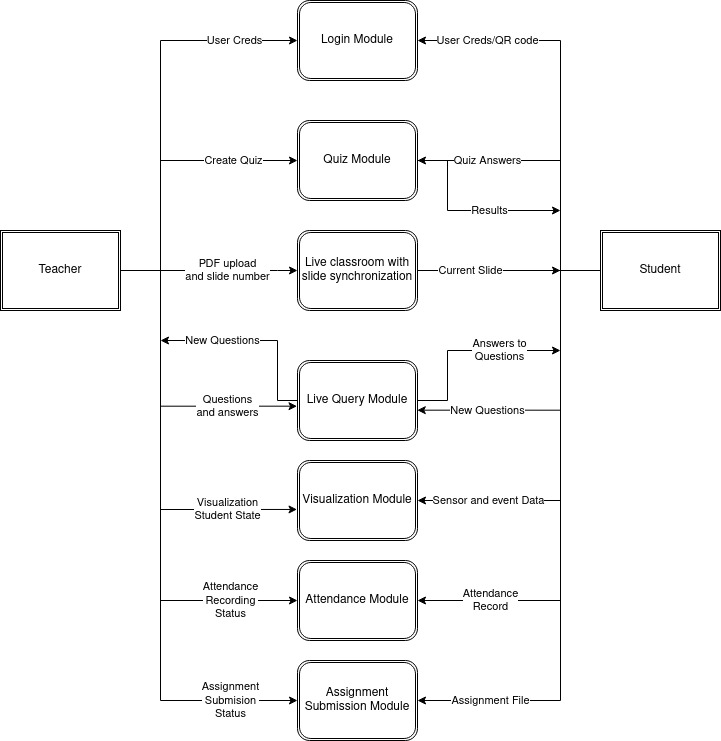
\includegraphics[width=\textwidth]{toplevel.jpeg} \newpage 
\paragraph{As explained in the previous chapter, the entire project can be divided into three parts, 1) An Android Application which acts as the interface, 2) Supporting Backend Scripts \& 3) Emotion AI Models to classify the learners' state. Understanding the entire system is tedious by individually reading either of these parts since all the parts run in sync. Understanding the system from the User Interface POV is easier since the end-user can identify the different components. From a UI perspective, the entire system can be divided into seven different modules. In this chapter, we will try to explain each module using their Data Flow Diagram to ease in the understanding of how the three parts work together in sync.}  
\section{User Registration \& Authentication Module}
Login Module is the first encountered UI. There are two types of users - students \& teachers. The teacher can login to his dashboard using the credentials provided to him by the administrator. Similary, a student can login into the system by using his credentials. However, a student needs to scan the QR before joining the classroom. This enables the system to understand the location at which the student sat down.  \\ \\ 
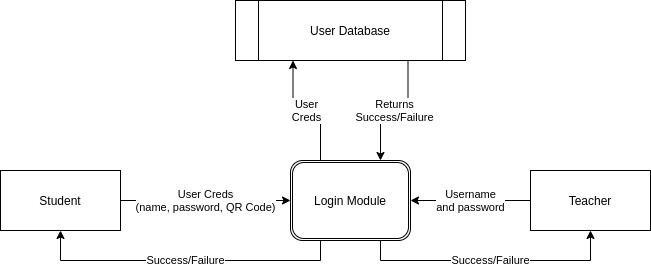
\includegraphics[width=\textwidth]{LoginModule.jpg}
\section{Virtual Classroom Module}
The Virtual Classroom for both the students and teacher is different. For a teacher, there is an option to generate text-based PDF, upload PDF files \& start a teaching session with an uploaded file. A Student has an option to join the virtual teaching session. As soon as the student joins the classroom, the PDF Viewer synchronizes with the teacher screen after fetching details from the server. The student doesn't need to store the file on his local mobile device due to option of Server-Side Storage. Once inside this discussion module, the teacher can switch to the Visualization Dashboard within this screen \& analyze the general state of the classroom. Similarly, a student can make notes while he is inside the virtual teaching session. 
\\ \\
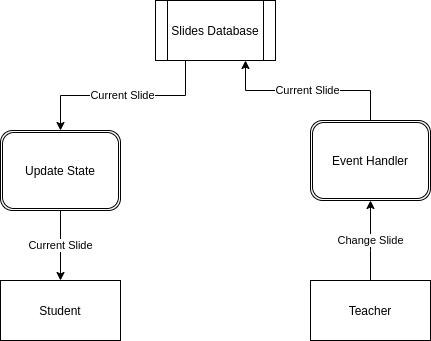
\includegraphics[width=\textwidth]{LiveClassroom.png}

\section{Live Discussion Module}
The live discussion module creates a query dashboard once the user is inside the virtual teaching session. A student can post queries related to the current slide which can be viewed by the teacher as well as the other students. All the other users can up-vote the questions whereas the teacher can respond to the query while teaching itself. The details of the likes \& comments on any query are stored on the server itself. They are fetched after the regular polling time interval of 5 seconds. 	\\ \\
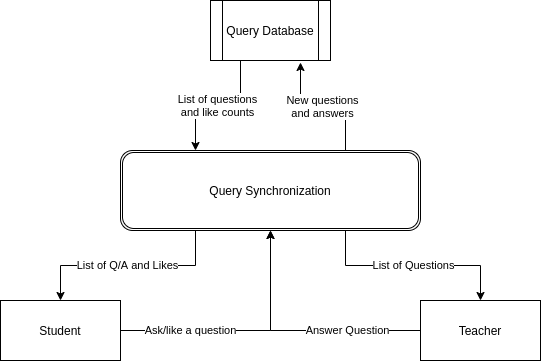
\includegraphics[width=\textwidth]{QuerySynchronization.png} \newpage
\section{Examination Module}
The Examination Module of the project can be used by the teacher to organize Quizzes for the logged in students inside the blended learning environment. The teacher has options to clear previous data, form new quizzes \& add new questions to the current quiz. The student can attempt the current quiz \& also view the score of his attempt after he finishes the quiz. A student has the option to revisit all the questions before submitting his responses. \\ \\
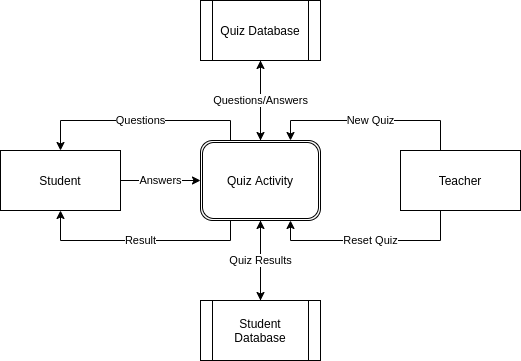
\includegraphics[width=\textwidth]{QuizModule.png} \newpage
\section{Visualization Module}
The Visualization Module is the most important module of the entire project. This enables the teacher to analyse the mental states of student which is shown to him in a presentable manner. When the teacher logs inside the Vedinkaksa System, he is asked to input the dimensions of the rectangular classroom which is then used by the Dynamic Visualization Algorithm to prepare an empty visualization model. When the students login to the system, the teacher is able to view their mental \& emotional states. A student can be recognized by his profile picture inside the Visualization Dashboard. \\ \\
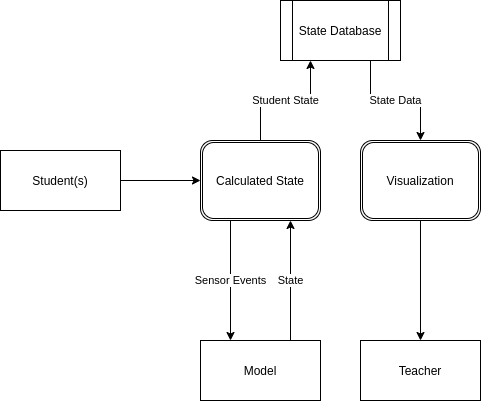
\includegraphics[width=\textwidth]{VisualizationModule.png}  
\section{Attendance Module}
The Attendance Module of the application was added to take in-app attendance. The teacher can start the attendance once he is logged inside the app. The students can use the Attendance Module inside their Dashboard to register their attendances while the teacher permits taking attendance. This system can be used by the teacher to analyze the general trend between the grades \& attendance of any student. \\ \\ 
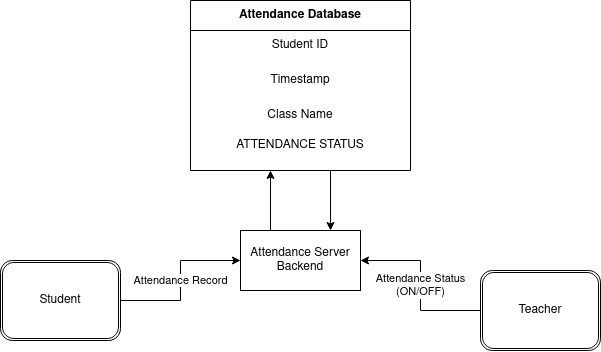
\includegraphics[width=\textwidth]{attendance.jpeg}   \newpage
\section{Assignments Module}
The Assignments Module of the app can be used for taking submissions within the class. The teacher can control the time for which submissions will be accepted whereas the student can submit their works \& see the reviews inside this module on their User Interface Screen. The Students can't submit a work once the teacher has stopped the submissions of assignments. This module uses Server-Side Storage of the files of the students and thus no one can modify the file except the administrator. \\ \\ 
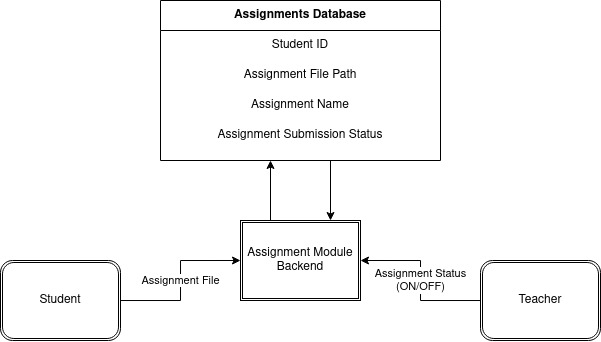
\includegraphics[width=\textwidth]{assignments.jpeg} 
\chapter{Contribution of the Authors}
\section{Introduction}
We have worked on the Vedinkaksa Project for the last two semesters. Our contribution to the project can be summarized as follows:
\begin{itemize}
\item{Debugging of the pre-existing system \& successfully deploying it.}
\item{Implementation of Server Side Storage for Virtual Classroom \& Query Synchronization.}
\item{Implementation of Dynamic Visualization from scratch \& integration of the Visualization Screen with Emotion AI Models to depict the correct user' states}
\item{Design \& Implementation of an Assignments Module within the Android App just like Moodle.}
\item{Implementation of an in-class Attendance Module within the Android App.}
\item{Writing an exhaustive Developers' Guide for easing the installation procedure in future.}
\end{itemize}  
In the upcoming sections, we will be going over our contributions to each module in a systematic way so that the report can also serve as a basic user manual in the future.  
\section{Virtual Classroom Module}
Inside the Virtual Classroom Module, the pre-existing application demanded the presence of the teaching file on the local devices of the educator as well as the learner. Many file system changes were made after Android 10 which made it difficult for the Vedinkaksa application to render the PDF stored inside the local directories of their mobile phones. Thus, we came up with the idea of a server side storage of files which would also reduce the latency of synchronization of slides since the clients would now be interacting with the server instead of each other. The capacity of server can be increased for further minimization of the latency. \\ \\
The pre-existing application contained the feature of slide synchronization which was based on client-client interactions. Once we decided to move to the server-client architecture, we came up with the idea of including a table inside the existing database which could be used for synchronizing the slides. A Record of the current slide and the current teaching material was inserted into the table. Whenever the teacher changes his slide number, an event gets triggered within the android application which updates the slide number accordingly. Instead of downloading the slide on the student device, the changed slide now gets streamed to all the active student devices. Due to the streaming feature, the student which joins the environment late will also be able to directly begin with the current slide instead of the first slide. \\ \\ 
The inclusion of a server side storage and a global slide-file table in the database eased the load on the client devices whereas the load on the server increases due to this. However, by increasing the processing capabilities of the server, the system will have reduced latencies for the synchronization of slides. Moreover, by removing the necessity to download the files on local client devices, a lot of device space has been conserved for the clients.          
\section{Visualization Module}
The pre-existing application had a visualization model using different static models. A dynamic Visualization model proposed by Dr. Samit Bhattacharya \& Mr. Ujjwal Biswas was incorporated into the application by us. As mentioned previously, an emotion AI model developed by Mr. Subrata Tikadar was present within the system. But the main challenge was to integrate with our visualization model. To include this feature, we implemented the backend support which called the trained AI function and returned the result of the mental state of the student after every 7 seconds as a json encoded string. We parsed this string \& fetched the student's details which came from the QR code used by the student. The fetched details were then used to correctly map the current user states to the visualization screen \& subsequently update them as per the algorithm.
\section{Assignments Module}
An assignments module was added into the system by us. In this module, the teacher can inform the students about the assignment during the class. As of now, the teacher interface can be used to open the submissions whereas a proper interface has been implemented for the students where they could submit their submissions and see their score. Assignments are an important part of the learning experience and the educator can use this forum to get continuous feedback of the learners. This module was implemented by using a server-side storage of assignments of each user. The control of the submission due date \& time is manual as of now and depends on the teacher. This was made successful by addition of a single entry table in the database which was updated as per the teacher.  
\section{Attendance Module}
The need of a proper attendance system was mandatory to understand the impact of scores of the students with their attendance. Thus, we felt the need to incorporate an in-app attendance module. The teacher can use this feature to control \& manage the attendance. The students can mark their attendance within the stipulated time for which the teacher opens the attendance module. The control of the attendance is manual \& needs to be managed by the teacher. To incorporate the controlling powers with the teacher, we decided to add a single entry table in the database which returned the current status of the attendance module.   
\section{Documentation Writing}
As written in the $2^{nd}$ chapter, the contribution of previous developers couldn't be ignored. However, the difference in coding style between different developers made it difficult for a new user to understand the flow of the application. Moreover, it wasn't even possible to deploy the application successfully because all the developers worked on different parts of the entire system \& the pre-existing deployment documentation was outdated and insufficient for successful setting up of the system. One of the major contributions of our entire work was also to write inline codes for some of the server files, debug pre-existing code \& write an exhaustive technical documentation which could be referred by future developers to deploy the system \& understand the code flow in no time.   
\chapter{Developers' Guide}
\section{Initial Server Setup}

\begin{itemize}

\item{Enabling SSH on Ubuntu}
\begin{itemize}
\item{sudo apt update}
\item{sudo apt install openssh-server}
\item{sudo systemctl status ssh - You should see something like Active: active (running) :}
\end{itemize}

\item{Give Firewall Access}
\begin{itemize}
\item{sudo ufw allow ssh}
\end{itemize}

\item{Find your public IP Address \& connect through SSH}
\begin{itemize}
\item{ip a}
\item{ssh username@ip\_address}
\end{itemize}

\item{Create a New User \& grant administrative privileges}
\begin{itemize}
\item{adduser sammy}
\item{usermod -aG sudo sammy}
\end{itemize}
\end{itemize}

\section{Setting up LAMP Stack}
\begin{itemize}
\item{Installing Apache and Updating the Firewall}
\begin{itemize}
\item{sudo apt update}
\item{sudo apt install apache2}
\item{sudo ufw app list - You’ll see output like this: \\
\textbf{Output}
Available applications:
Apache
Apache Full
Apache Secure
OpenSSH}
\item{sudo ufw allow in "Apache"}
\\ You can verify the change with:
\item{sudo ufw status}
\end{itemize}
You can do a spot check right away to verify that everything went as planned by visiting your server’s public IP address in your web browser
http://your-server-ip 
\item{Installing MySQL}
\begin{itemize}
\item{sudo apt install mysql-server}
\item{sudo mysql\_secure\_installation} \\
This will ask if you want to configure the VALIDATE PASSWORD PLUGIN.Regardless of whether you chose to set up the VALIDATE PASSWORD PLUGIN, your server will next ask you to select and confirm a password for the MySQL root user. This is not to be confused with the system root. The database root user is an administrative user with full privileges over the database system. When you’re finished, test if you’re able to log in to the MySQL console by typing:
\item{sudo mysql} \\
This will connect to the MySQL server as the administrative database user root, which is inferred by the use of sudo when running this command.
\end{itemize}
\item{Installing PHP}
\begin{itemize}
\item{sudo apt install php libapache2-mod-php php-mysql}
\\ Once the installation is finished, you can run the following command to confirm your PHP version:
\item{php -v} 
\\ \textbf{Output}
PHP 7.4.3 (cli) (built: Mar 26 2020 20:24:23) ( NTS )
Copyright (c) The PHP Group
\end{itemize}
\item{Creating a Virtual Host for your Website}
\begin{itemize}
\item{sudo mkdir /var/www/your\_domain} \\
Next, assign ownership of the directory with the \$USER environment variable, which will reference your current system user:
\item{sudo chown -R \$USER:\$USER \/var\/www\/your\_domain} \\
Then, open a new configuration file in Apache’s sites-available directory using your preferred command-line editor. Here, we’ll use nano:
\item{sudo nano /etc/apache2/sites-available/your\_domain.conf} \\
This will create a new blank file. Paste in the following bare-bones configuration:
\item{$\langle$ VirtualHost *:80 $\rangle$ \\
ServerName your\_domain \\
ServerAlias www.your\_domain \\
ServerAdmin webmaster\@localhost \\
DocumentRoot \/var\/www\/your\_domain \\
ErrorLog \$\{APACHE\_LOG\_DIR\}/error.log \\
CustomLog \$\{APACHE\_LOG\_DIR\}/access.log combined \\ 
$\langle$/VirtualHost $\rangle$} \\ \\ 
Save and close the file when you’re done. With this VirtualHost configuration, we’re telling Apache to serve your\_domain using
/var/www/your\_domain as the web root directory.
\end{itemize}
\end{itemize}
\section{Installing and Securing phpMyAdmin on Ubuntu}
\begin{itemize}
\item{Installing phpMyAdmin}
\begin{itemize}
\item{sudo apt update}
\item{sudo apt install phpmyadmin php-mbstring php-zip php-gd php-json php-curl} \\
For the server selection, choose apache2. Then, open up your MySQL prompt \& execute the following commands.
\item{mysql -u root -p}
\item{UNINSTALL COMPONENT " file://component\_validate\_password ";}
\item{exit}
\item{sudo apt install phpmyadmin}
\item{INSTALL COMPONENT " file://component\_validate\_password ";}
\item{exit}
\item{sudo phpenmod mbstring}
\item{sudo systemctl restart apache2}
\end{itemize}
\item{Adjusting User Authentication and Privileges} \\ 
When you installed phpMyAdmin onto your server, it automatically created a database user called phpmyadmin which performs certain underlying processes for the program. Rather than logging in as this user with the administrative password you set during installation, it’s recommended that you log in as either your root MySQL user or as a user dedicated to managing databases through the phpMyAdmin interface. In order to log in to phpMyAdmin as your root MySQL user, you will need to switch its
authentication method from auth\_socket to one that makes use of a password, if you haven’t already done so. \\ To do this, execute the following commands:
\begin{itemize}
\item{sudo mysql}
\item{
ALTER USER 'root'@'localhost' IDENTIFIED WITH caching\_sha2\_password BY 'password';}
\item{
ALTER USER 'root'@'localhost' IDENTIFIED WITH mysql\_native\_password BY 'password';} \\
Then, check the authentication methods employed by each of your users again to confirm that root no longer authenticates using the auth\_socket plugin:
\item{SELECT user,authentication\_string,plugin,host FROM mysql.user;}
\end{itemize}
\item{Configuring Password Access for a Dedicated MySQL User}
\\ Use the same commands as shown below exclusively:
\begin{itemize}
\item{mysql -u root -p}
\item{
CREATE USER 'nikhil'@'localhost' IDENTIFIED WITH caching\_sha2\_password BY '160101047';}
\item{
ALTER USER 'nikhil'@'localhost' IDENTIFIED WITH mysql\_native\_password BY '160101047';}
\item{
GRANT ALL PRIVILEGES ON *.* TO 'nikhil'@'localhost' WITH GRANT OPTION;}
\item{
exit}
\\ You can now access the web interface by visiting your server’s domain name or public IP address followed by /phpmyadmin.
\end{itemize}
\end{itemize}
\newpage
\section{Training the Model}
\begin{itemize}
\item{Copy the server directory from the Project Folder and place it in the PHP site folder in your computer. For Linux: /var/www/your\_domain/Sites}
\item{To check that the Server folder has been copied correctly, nautilus into that directory, put a test.php file in that directory of your server \& try to open http://server\_ip/test.php . If the file is working correctly, proceed ahead. Otherwise, return to Step 1 of Training the Model.}
\item{Open phpMyAdmin as described earlier and import (Import -> Choose
File) all the files, in the database directory while leaving all options set as default.}
\item{Next, Create a virtual environment for Python3, using the venv
package, for creating an isolated environment for running the models. Use the following commands:}
\begin{itemize}
\item{python3 -m venv myenv}
\item{
source myenv/bin/activate}
\end{itemize}
\item{Now, go to the Models directory within the virtual environment \& run the models using \\ python3 main.py}
\\
Some packages like numpy, panda, etc need to be installed in the virtual environment. It is suggested to try to execute the file using the above command \& manually install all the files which the interpreter asks you to install. It will ask you to install all the packages line by line as included in the main.py file. Once all the basic requirements are met, we are ready to proceed ahead. Once the file is executed, note that the line “Iteration xx completed” should pop in the terminal within 1-2 seconds after executing the python file. If it doesn’t run within
this time frame, something must be wrong. 
\item{Once the initial training is over \& iterations start, it is supposed to let this terminal process run in the background \& move ahead with building the mobile app.}
\end{itemize}
\newpage
\section{Installing Android Studio}
\begin{itemize}
\item{sudo apt install openjdk-11-jdk}
\item{sudo add-apt-repository ppa:maarten-fonville/android-studio}
\item{sudo apt update}
\item{sudo apt install android-studio}
\item{Launch Android Studio} \\ 
Go to the Application Launcher Bar \& launch it by pressing the Android Studio Icon. Do not import Settings \& accept the licenses. Use the standard Setup settings provided by Android Studio. Wait for all the components to be installed before the main screen appears. \\ \\ 
\textbf{Note:} Once all the components have been installed, go to Configure -$\rangle$ SDK Manager -$\rangle$ SDK Tools \& install the necessary licenses \& tools for SDK version starting with 28. By default, only the latest version is installed. Ensure that SDK Version starting with 28 is installed along with the latest version as it may produce some errors if that particular version hasn’t been installed.
\end{itemize}
\newpage
\section{Deploying the Mobile Application}
\begin{itemize}
\item{Open the project folder in Andorid Studio. It will start indexing the files which may take some time depending on processor speeds and RAM.}
\item{Replace the IP in the server field with your server\_ip, in the Constants.java file (java/iitg/vedinkaksa/Constants.java) in the Android Project. Remember that this is the same IP which was used while setting up Ubuntu Server.}
\item{Build the APK once Android Studio \& it’s components have been installed in the configuration described above.}
\item{Run the application. (It is suggested to run the application on your mobile device instead of the emulator if your RAM is less than 16GB).}
\item{The credentials for logging in has been provided in the Credentials Folder. QR Codes are also present in the same folder which will let the students log in to the application.}
\item{Use the logcat in Android Studio to debug in case of basic error. If any error with the Error Code 404 comes in the logcat, ensure that the path to that file is correct.}
\end{itemize}
\textbf{Note:} If you are running the app on your mobile device, ensure that the linux server \& mobile device are on the same Wifi. If this condition is not met, you won’t be able to log in to the app.
\newpage
\section{Iterating over the Models}
The python State detection models are independent of the Android App. Thus, iterating upon the model would not require you to recompile the Android APK (unless the server IP is changed). However, you are required to restart the Python server. \\ \\
There are different functions corresponding to each model in the Code (in
models/classifier/classifier/main.py). In order to update any model, please
change code in the function corresponding to that model. \\ \\
Before restarting the server, please verify that the path to the training data for each model has been specified correctly in the corresponding functions. Finally, interrupt the server (ctrl + C), in case it’s already running, and then restart the server using the commands given under Training the Models.
\chapter{Conclusion \& Future Works}

Vedinkaksa was developed with the vision of limiting the gap between the educator and the learner. We believe that we have been able to bring the existing system into a state where there are more than one ways to do so. We have tried to limit the bugs and errors to as less as we could. In our opinion, making an existing feature bug-free is as important as the inclusion of a new feature. In the course of two semesters, we have not only tried to incorporate new changes but also went on to resolve existing bugs in the system. At the time when this report is being written, some of the features of this system have been tested successfully on 7-8 devices simultaneously by the help of of Dr. Samit Bhattacharya \& Mr. Ujjwal Biswas. Rest of the features have been tested by us on 3-4 devices and everything worked seemlessly. We expect the entire system to work in coherence on any server. \\ \\
During the development, we focussed on unit testing. Unit testing of any system is important to understand the faulty module/unit. Although the code for Emotion AI Models were already written, we independently verified the sensor data such as touch, type \& involvement data. Similarly, we checked the code of dynamic visualization initially with random classroom sizes and when we found both the separate units to be correctly working, we integrated them \& the Visualization module came to it's present shape. \newpage
With the advancement of technology, the file system of Android OS changed which made it difficult to go on with the pre-existing virtual classroom module. The current implementation of a Server-Side Storage for teaching materials is a result of the same. This development is a crucial part of the system as it reduces the load on individual clients is concerned. The same idea of having a server-side storage also helped us to expand the application \& implement an Assignments Module which can be used by the educators to ask for submissions within a stipulated time period.
\section{Scope of Future Works}
With the improvement of technology \& increasing cases of Covid-19, the usage of digital mediums for teaching is getting popular. Blended Learning is a western concept which intends to improve the teaching culture for better learning of the students. Vedinkaksa, which is based on Human Computer Interaction is one of the very first works in this domain as per our knowledge \& thus the scope of future works in intense.
A good model based on affective computing is present with us. However, one can certainly come up with better models to do so. Similarly, presenting the visualization data to the teacher is currently possible for a rectangular classroom only. A Visualization Scheme for different shapes of classroom can be considered as a future work in this project. Moreover, features such as Interactive Live Group Discussion can be integrated with the Android Application. NLP \& other Deep Learning Models can be used to understand the mental state of a student by analysing the text written by him/her. Another challenge which comes up with blended/online modes of teaching is co-relating the learning by assessment(quiz) results due to cheating. An Anti-Plag sub-module can be incorporated within the Examinations Module of the Vedinkaksa system to tackle the same. \\ \\
Summing up the above, there are a lot of ideas \& things to improve the entire blended learning platform. Through Vedinkaksa, we have tried to address some of those \& implemented them into a full-fledged working prototype.  
\begin{thebibliography}{4}
\bibitem{stsb}	Subrata Tikadar and Samit Bhattacharya. "A novel method to build and validate an affective state prediction model from touch-typing",
\emph{In David Lamas, Fernando Loizides, Lennart Nacke, Helen Petrie, Marco Winckler, and Panayiotis Zaphiris, editors, Human-Computer Interaction – INTERACT 2019, pages 99–119, Cham, 2019. Springer International Publishing.}
\bibitem{stsbvt}	S. Tikadar, S. Bhattacharya, and V. Tamarapalli. "A blended learning platform to improve teaching-learning experience", \emph{In 2018 IEEE 18th International Con- ference on Advanced Learning Technologies (ICALT), pages 87–89, 2018.}
\bibitem{sbub}	Samit Bhattacharya, Viral Bharat Shah, Krishna Kumar, and Ujjwal Biswas. 2019. "A Real-time Interactive Visualizer for Large Classroom", \emph{J. ACM 1, 1, Article 1 (January 2019), 27 pages. https://doi.org/10.1145/1122445.1122456}
\bibitem{and}	"Android documentation", \emph{https://developer.android.com/docs.}
\end{thebibliography}  
\end{document}
